\begin{center}\Large\textbf{Readings 9.1-9.5%Rao Readings: 9.1-9.5 326-360}
}\\
\normalsize \end{center}
\large ~\hrulefill
~\\\textit{\textcolor{blue}{For the next section or two we will continue to consider experiments that have a quantitative response and categorical predictors only (i.e. experiments that can be analyzed using One-Way ANOVA).  To start with let`s just look at a completely randomized experimental design (i.e. all treatments are randomly assigned to the experimental units).  We will look at contrasts of the parameters that will lead directly into the way to analyze Multi-Way ANOVA models where a `factorial' treatment structure is used.}}\\~\\~\\

Consider the traditional balanced One-Way ANOVA model (\textbf{ANOVA (Analysis of Variance, i.e. comparing mean squares)}).  That is,
\begin{itemize}
\item we have a \textit{continuous} response, $Y$
\item \textit{qualitative or categorical} predictor(s) which we call our \textbf{factor(s)} (often we will use a continuous factor that is only observed at a few values as our categorical factor)
\item if a single factor then the \textbf{levels} of the factor are our \textbf{treatments}, if multiple factors the combinations of levels from the factors is the treatment. (Either way, $t$ = total number of treatments)
\end{itemize}
(One-Way corresponds to having only one factor of interest.)\\~\\

\newpage

One form of the One-Way ANOVA model is
$$Y_{ij}=\mu_{i}+E_{ij}$$
\begin{itemize}
\item $E_{ij}$ are iid $N(0,\sigma^2)$
\item $i=1,...,t$ describes the treatment group
\item $j=1,...,n_i$ represents the number of replications we have in treatment group $i$. 
\end{itemize}
We will consider `balanced' designs for now, where $n_i=n$, same number of replicates for each treatment.  Total number of observations = $N = nt$\\~\\


\textbf{Unknown parameters:}
\begin{itemize}
\item $\mu_{i}$ - (true) mean response for all members of population $i$\\
Estimate:\\~\\~\\~\\
\item $\sigma^2$ - (true) variance within a given treatment group (assumed constant across groups)\\
Estimate:\\~\\~\\~\\~\\~\\
\end{itemize}

\textbf{Goals of One-Way ANOVA}: Determine
\begin{enumerate}
\item if all treatment group means are equal.\\~\\
\item if treatment group means are not equal, which means differ from each other.
\end{enumerate}

\newpage

\textbf{One-Way ANOVA example}:\\
An experiment was done to determine if there was a difference between antibiotic types in terms of their mean binding fraction in bovines.  \\
There were N=20 bovines that were randomly assigned to one of t=5 types of antibiotics (the levels of the factor, since only one factor these levels are also the treatments), yielding n=4 replicates for each treatment. \\
The data given here, labeled in terms of the One-Way ANOVA format:
\begin{center}
\begin{tabular}{lc|cc} 
Binding Fraction (Y) & Antibiotic& True Trt Mean & Sample Mean\\\hline
$y_{11}=29.2$ & Chloramphenicol&\multirow{4}{*}{$\mu_1$}&\multirow{4}{*}{$\bar{y}_{1\bullet}=27.8$}\\
$y_{12}=32.8$ & Chloramphenicol\\
$y_{13}=25.0$ & Chloramphenicol\\
$y_{14}=24.2$ & Chloramphenicol\\\hline
$y_{21}=21.6$ & Erythromycin&\multirow{4}{*}{$\mu_2$}&\multirow{4}{*}{$\bar{y}_{2\bullet}=19.1$}\\
$y_{22}=17.4$ & Erythromycin\\
$y_{23}=18.3$ & Erythromycin\\
$y_{24}=19.0$ & Erythromycin\\\hline
$y_{31}=29.6$ & Penicillin G &\multirow{4}{*}{$\mu_3$}&\multirow{4}{*}{$\bar{y}_{3\bullet}=28.6$}\\
$y_{32}=24.3$ & Penicillin G \\
$y_{33}=28.5$ & Penicillin G \\
$y_{34}=32.0$ & Penicillin G \\\hline
$y_{41}=5.8$ & Streptomycin&\multirow{4}{*}{$\mu_4$}&\multirow{4}{*}{$\bar{y}_{4\bullet}=7.8$}\\
$y_{42}=6.2$ & Streptomycin\\
$y_{43}=11.0$ & Streptomycin\\
$y_{44}=8.3$ & Streptomycin\\\hline
$y_{51}=27.3$ & Tetracyclin&\multirow{4}{*}{$\mu_5$}&\multirow{4}{*}{$\bar{y}_{5\bullet}=31.4$}\\
$y_{52}=32.6$ & Tetracyclin\\
$y_{53}=30.8$ & Tetracyclin\\
$y_{54}=34.8$ & Tetracyclin\\\hline
\multicolumn{4}{l}{$\bar{y}_{\bullet\bullet}=22.9$}\\
\end{tabular}
\end{center}

\textcolor{blue}{Recall:  Notation for means in One-Way ANOVA -\\
Overall sample mean = $\bar{y}_{\bullet\bullet}$ or $\bar{y}_{++}$ (mean over index i and index j)\\~\\~\\~\\
Treatment $i$ sample mean = $\bar{y}_{i\bullet}$ or $\bar{y}_{i+}$ (mean over index i)}\\~\\~\\~\\~\\

Goal: Test if the population means for these 5 treatments are plausibly equal. \\
If not equal, which treatment means differ significantly? 

\newpage

\textbf{Modeling the binding fraction experiment:}\\
One-Way ANOVA model is appropriate: 
$$Y_{ij} = \mu_i + E_{ij}$$
for $i=1,\ldots,5$ and $j=1,\ldots,4$, where $E_{ij}$ are i.i.d. $N(0,\sigma^2)$ errors.
\begin{eqnarray*}
\mu_1 & = & \mbox{mean of Cholramphenicol treatment}\\
\mu_2 & = & \mbox{mean of Erythromycin treatment}\\
\vdots\\ 
\mu_5 & = & \mbox{mean of Tetracyclin treatment}
\end{eqnarray*}
~\\~\\
To test 
$H_0:$\\~\\ %$$\mu_1 = \mu_2 = \ldots = \mu_5$$
vs\\~\\
$H_A:$\\~\\ %\mbox{ at least 1 mean differs}$$
we use software to compute the One-Way ANOVA table and look at `global' p-value from the table.\\~\\
\textbf{Table for balanced one-way ANOVA:}
\begin{center}
\begin{tabular}{|c|c|c|c|c|c|} \hline
Source & DF & SS & MS & F & P-value\\ \hline
Treatments & $t-1$ & $SS(T)$ & $MS(T)=\frac{SS(T)}{(t-1)}$ & $F=\frac{MS(T)}{MS(E)}$ & $P(F_{t-1,t(n-1)}>F_{obs})$\\ 
Error & $t(n-1)$ & $SS(E)$ & $MS(E)=\frac{SS(E)}{(N-t)}$ & &\\
Total & $nt-1$ & $SS(Tot)$ & & &\\ \hline
\end{tabular}
\end{center}
where
\begin{eqnarray*}
SS(T) & = &\sum_{i=1}^{t} \sum_{j=1}^{n} (\bar{y}_{i\bullet} - \bar{y}_{\bullet\bullet})^2 = n\sum_{i=1}^{t}(\bar{y}_{i\bullet} - \bar{y}_{\bullet\bullet})^2\\
SS(E) & = & \sum_{i=1}^{t} \sum_{j=1}^{n}(y_{ij}-\bar{y}_{i\bullet})^2 \\
SS(Tot)&=& \sum_{i=1}^{t} \sum_{j=1}^{n}(y_{ij}-\bar{y}_{\bullet\bullet})^2
\end{eqnarray*}
Note:  SS(T) is also called SS(Between) and SS(E) is also called SS(Within).

\newpage

In SAS, 
\begin{small}
\begin{verbatim}
proc glm data=binding;
class antibiotic;
model bindfrac=antibiotic;
means antibiotic;
run;
\end{verbatim}
\end{small}
\begin{center}
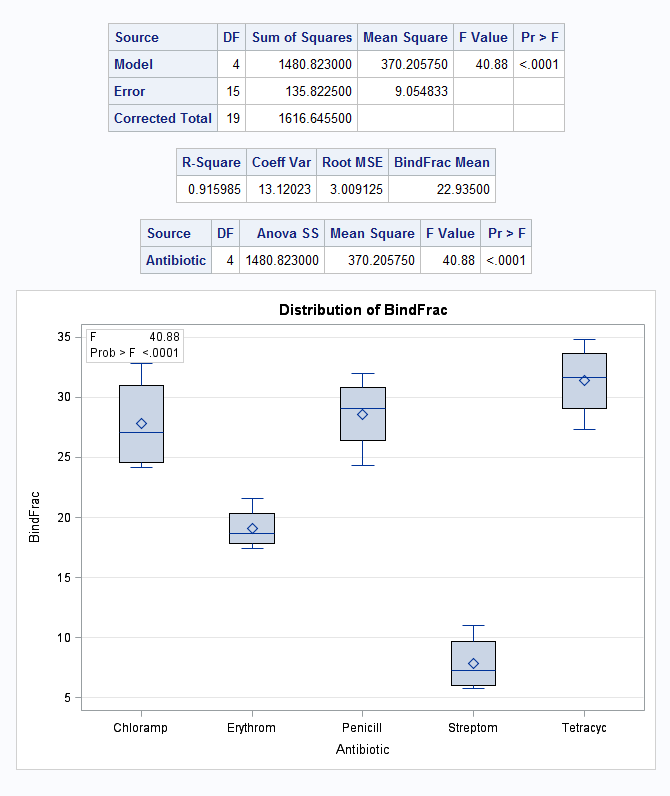
\includegraphics[scale=0.6]{BindFracANOVA}\includegraphics[scale=0.4]{BindFracBoxplot2}\\
\end{center}

Conclusion about treatment means begin equal?\\~\\~\\~\\~\\~\\

%\textcolor{red}{p-value $<$ 0.05 so reject $H_0$ in favor of $H_A$.  That is, at the 5\% S.L. there is enough evidence to say at least one antibiotic differs in terms of binding fraction.}\\~\\
%The next step is to do pairwise comparisons of means using a multiple comparison correction.  We will take this up shortly.\\~\\

\newpage

\Large\textbf{Given the answer to the previous question, the next logical question to answer is: `Which treatment means are different?'}\large \\

Suppose we want first inspect the difference between the Cholramphenicol ($\mu_{1}$) and Erythromycin treatment means ($\mu_{2}$).  In terms of $\mu_{1}$ and $\mu_{2}$, how can we write this question as a null and alternative hypotheses?\\~\\~\\~\\~\\
%\color{red}{$$H_{0}: \mu_1-\mu_2=0~~~\mbox{or}~~~\mu_1=\mu_2~~vs~~H_{A}:\mu_1-\mu_2\neq 0~~~\mbox{or}~~~\mu_1\neq\mu_2$$}

We get an estimator this quantity with the corresponding sample means\\~\\~\\~\\
%$$\hat{\mu}_{1}-\hat{\mu}_{2}=\bar{Y}_{1\bullet}-\bar{Y}_{2\bullet}$$~\\

The standard error of this quantity can be found by taking the square root of the variance (recall we assume our samples are independent so covariance is 0)\\~\\~\\~\\~\\~\\~\\
%$$Var(\bar{Y}_{1\bullet}-\bar{Y}_{2\bullet}) = (1^2)Var(\bar{Y}_{1\bullet})+(-1)^2\bar{Y}_{2\bullet}+2(1)(-1)Cov(\bar{Y}_{1\bullet},\bar{Y}_{2\bullet})$$
%$$=Var(Y_{1j})/n_1+Var(Y_{2j})/n_2 = \sigma^2/n_1+\sigma^2/n_2$$~\\

For a balanced design we have\\~\\~\\~\\~\\
%$$Var(\bar{Y}_{1\bullet}-\bar{Y}_{2\bullet}) = \sigma^2(1/n+1/n) = 2\sigma^2/n$$
yielding a standard error of\\~\\~\\~\\~\\
%$$SE(\bar{Y}_{1\bullet}-\bar{Y}_{2\bullet})=\sqrt{2\sigma^2/n}$$~\\

By the normality assumption on the data we then have a case similar to the two-sample t test with pooled variance!\\~\\
$$\bar{Y}_{1\bullet}-\bar{Y}_{2\bullet}\sim N(\mu_1-\mu_2,\sigma^2(1/n_1+1/n_2)) = N(\mu_1-\mu_2,2\sigma^2/n) $$~\\

We estimate $\sigma^2$ by the common pooled estimate (over all the samples, not just these two)
$$MS(E)=S^2_w=\frac{SS(E)}{t(n-1)}=\frac{\sum_{i=1}^{t}\sum_{j=1}^{n}(Y_{ij}-\bar{Y}_{i\bullet})^2}{N-t}$$~\\

Thus, we can for a t-test for testing $H_0:\mu_1=\mu_2~~~vs~~~H_A:\mu_1\neq\mu_2$ using
$$T=\frac{\bar{Y}_{1\bullet}-\bar{Y}_{2\bullet}}{\sqrt{MS(E)(1/n_1+1/n_2)}}=\frac{\bar{Y}_{1\bullet}-\bar{Y}_{2\bullet}}{\sqrt{2MS(E)/n}}\sim t_{N-t}=t_{t(n-1)}$$~\\~\\
We can form a $(1-\alpha)100\%$ CI for $\mu_1-\mu_2$ using
$$\bar{Y}_{1\bullet}-\bar{Y}_{2\bullet}\pm t_{\alpha/2,N-t}\sqrt{MS(E)(1/n_1+1/n_2)}~~~or~~~\bar{Y}_{1\bullet}-\bar{Y}_{2\bullet}\pm t_{\alpha/2,N-t}\sqrt{2MS(E)/n}$$
and check if 0 is in the interval.\\~\\~\\~\\
\begin{enumerate}
\item Create a 95\% CI for $\mu_1-\mu_2$ ($P(T_{15}>2.13)=0.025$) and also find the test statistic for testing the above hypotheses.   What is your conclusion?
\end{enumerate}

\newpage

\Large\textbf{More generally than just wanting to see which means differ, we may want to compare different functions of means.}\large\\~\\
The functions of the means will be in the form of a \textbf{linear combination} of the treatment means.\\
In general, a linear combination of treatment means takes the form\\~\\~\\~\\~\\~\\
%\color{red}{$$\theta=c_{1}\mu_{1}+c_{2}\mu_{2}+...+c_{t}\mu_{t}$$
%where the $c_{i}$ are called the coefficients of the linear combination.}

For the bovine experiment, which of the following are linear combinations of treatment means?
\begin{itemize}
    \item $\theta_6=4\mu_{1}+3\mu_{2}-7\mu_{5}$\\ %yes
    \item $\theta_7=3\mu_{1}\mu_{4}+2\mu_{3}$ \\    %no
    \item $\theta_8=\mu_{1}+\mu_{2}+\mu_{3}+\mu_{4}+\mu_{5}$\\  %yes
    \item $\theta_9=\mu_{1}^2+3\mu_{2}+1$\\   %no
\end{itemize}
If the coefficients of the linear combination sum to zero the linear combination is called a \textbf{contrast}.\\~\\~\\~\\~\\
%i.e. $c_1+c_2+...+c_t=0$ or $\sum_{i=1}^{t}c_i=0
Is our linear combination $\mu_1-\mu_2=0$ a contrast?  How about any of $\theta_6$ through $\theta_9$?\\~\\~\\~\\~\\~\\

\newpage

If we want to do inference about a linear combination of treatment means we need an estimator of $\theta$, call it $\hat{\theta}$ and we will also need a measure of variability, say $\hat{SE}(\hat{\theta})$.\\~\\
An estimator is given by substitution of the sample means: 
    $$\hat{\theta}=c_{1}\bar{Y}_{1\bullet}+c_{2}\bar{Y}_{2\bullet}+...+c_{t}\bar{Y}_{t\bullet}$$
 Use the output from previous to estimate the following linear combinations:  \\~\\
    $$\theta_1=\mu_1~~~~\hat{\theta}_1=\underline{~~~~~~~~~~~~~~~~~~~~~~~~~~~~~~~~~~~~~~~~~~~~~~~}$$~\\
    $$\theta_2=\mu_2~~~~\hat{\theta}_2=\underline{~~~~~~~~~~~~~~~~~~~~~~~~~~~~~~~~~~~~~~~~~~~~~~~}$$~\\
    $$\theta_5=\mu_5~~~~\hat{\theta}_5=\underline{~~~~~~~~~~~~~~~~~~~~~~~~~~~~~~~~~~~~~~~~~~~~~~~}$$~\\
    $$\theta_6=4\mu_{1}+3\mu_{2}-7\mu_{5}~~~~\hat{\theta}_6=\underline{~~~~~~~~~~~~~~~~~~~~~~~~~~~~~~~~~~~~~~~~~~~~~~~~~~~~~~~}$$~\\
    $$\theta_8=\mu_{1}+\mu_{2}+\mu_{3}+\mu_{4}+\mu_{5}~~~~\hat{\theta}_8=\underline{~~~~~~~~~~~~~~~~~~~~~~~~~~~~~~~~~~~~~~~~~~~~~~~~~~~~~~~}$$

We now have a point estimate of the quantity in our null hypothesis, in order to conduct our test we must also know about the variability of this estimate, i.e. What is $\hat{Var}(\hat{\theta})$ or $\hat{SE}(\hat{\theta})$?\\~\\
The variance of a linear combination of means in One-way ANOVA has a very nice form:

\newpage

% \color{red}{
%$$Var(\hat{\theta})=\frac{c_{1}^{2}}{n_{1}}\sigma^2+\frac{c_{2}^{2}}{n_{2}}\sigma^2+...+\frac{c_{t}^{2}}{n_{t}}\sigma^2=\sigma^{2}\sum_{i=1}^{t}\frac{c_{i}^2}{n_{i}}$$
%This variance involves the unknown quantity $\sigma^2$.  What value can we use to estimate $\sigma^2$?
%$$\hat{Var}(\hat{\theta})=MS(E)\sum_{i=1}^{t}\frac{c_{i}^2}{n_{i}}$$
%We can then estimate the standard error by
%$$\hat{SE}(\hat{\theta})=\sqrt{MS(E)\sum_{i=1}^{t}\frac{c_{i}^2}{n_{i}}}$$}

\Large\textbf{Making inference about the linear combination: (includes contrasts)}\large\\
Due to the normality assumption each mean has a normal distribution and further, the linear combination will also have a normal distribution.  Therefore, once we estimate the variance, we can use a t-test and a t-interval.\\~\\~\\~\\
Let $\theta_0$ be a value of interest for our contrast (often 0). \\
To test $H_{0}:\theta=\theta_{0}$ vs $H_{A}:\theta\neq \theta_{0}$ we can use
        $$t=\frac{\hat{\theta}-\theta_{0}}{\hat{SE}(\hat{\theta})}\sim t_{t(n-1)}~\text{under}~H_{0}$$~\\
				
A $(1-\alpha)100$\% CI for $\theta$ is
$$\hat{\theta}\pm t_{\alpha/2,t(n-1)}\hat{SE}(\hat{\theta}) = \sum_{i=1}^{t}c_{i}\bar{y}_{i\bullet}\pm t_{\alpha/2,t(n-1)}\sqrt{MS(E)\sum_{i=1}^{t}\frac{c_{i}^2}{n_{i}}}$$~\\

What is the value of this test statistic and a 95\% CI for the $\theta_8$?  Compare the test stat to $t_{0.025,15}=2.13$ to make a conclusion.  What is your interpretation?

\newpage

\Large \textbf{Getting the answers from SAS}\large\\~\\
\textbf{Pairwise Contrasts in SAS}\\
Note:  A contrast that has only two nonzero $c$'s is called a \textbf{pairwise contrast} (as it looks at only two means). \\ These can be had easily in proc glm using the code below.\\~\\
Recall, if our global p-value is significant then our secondary goal is to find which means differ.  This question is answered via looking at all pairwise comparisons (contrasts) of means.
\\~\\
A \textbf{complex} contrast is a contrast that involves more than two non-zero coefficients.  For example, $\theta_{10}=\frac{\mu_{1}+\mu_{2}}{2}-\frac{\mu_{3}+\mu_{4}}{2}$ is a complex contrast.  \\~\\

\begin{small}
\begin{verbatim}
proc glm data=binding;

class antibiotic;

model bindfrac=antibiotic;

means antibiotic/ lsd cldiff lines;

lsmeans antibiotic/stderr pdiff;

run;
\end{verbatim}
\end{small}
~\\~\\~\\
*Generally we'll want to use lsmeans not means, but ok here since no covariates involved and a balanced design was done. (To be discussed more later.)
\begin{center}
\includegraphics[scale=0.65,page=4,trim=60mm 0mm 30mm 0mm ]{BindFracContrasts}\includegraphics[scale=0.65,page=5,trim=30mm 0mm 60mm 0mm ]{BindFracContrasts}\\
\includegraphics[scale=0.65,page=6,trim=60mm 80mm 30mm 0mm ]{BindFracContrasts}\includegraphics[scale=0.65,page=8,trim=30mm 80mm 60mm 0mm ]{BindFracContrasts}
\end{center}

Use the output to construct a 95\% CI for $\theta_{10}$.

\newpage
\textbf{Any linear combination in SAS.}\\
To get the estimate for $\theta_{10}$ (and a few other linear combinations of means) in SAS we can use proc glm or use proc mixed.\\~\\

Using the estimate and contrast statements in One-Way ANOVA:\\
We need to write our contrast in terms of the model parameters $\mu$, $\tau_1, \tau_2,\tau_3$, $\tau_4$, and $\tau_5$ (the alternative parameterization of the model, $Y_{ij}=\mu+\tau_i+E_{ij}$). \\~\\

For instance, 
$$\theta_{10}=\frac{1}{2}(\mu_1+\mu_2)-\frac{1}{2}(\mu_3+\mu_4)=\frac{1}{2}(\mu+\tau_1+\mu+\tau_2-(\mu+\tau_3+\mu+\tau_4))$$
$$=0\mu+\frac{1}{2}\tau_1+\frac{1}{2}\tau_2-\frac{1}{2}\tau_3-\frac{1}{2}\tau_4$$
In terms of syntax, we write contrast or estimate followed by a name to distinguish it.  Then we do
\begin{center}
intercept \underbar{coef on $\mu$}~~~treatment \underbar{coef on $\tau_1$}~~\underbar{coef on $\tau_2$}~~\underbar{coef on $\tau_3$}~~\underbar{coef on $\tau_4$}~~~\underbar{coef on $\tau_5$}
\end{center}
A contrast statements will give you the contrast sum of squares and a p-value.\\~\\
An estimate statement will estimate any `estimable' function of parameters and a p-value. \\~\\~\\



\begin{small}
\begin{verbatim}
proc glm data=binding;
class antibiotic;
model bindfrac=antibiotic/clparm;
estimate 'lsmean for trt 2'                 intercept 1 antibiotic 0 1 0 0 0;
estimate 'avg of trt 2 and trt 3 mean'      intercept 2 antibiotic 0 1 1 0 0/divisor=2;
estimate 'trt 1 vs trt 5'                   intercept 0 antibiotic 1 0 0 0 -1;
estimate 'avg of 1 and 2 vs avg of 3 and 4' intercept 0 antibiotic 1 1 -1 -1 0/divisor=2;
run;



proc mixed data=binding;
class antibiotic;
model bindfrac=antibiotic;
lsmestimate antibiotic 'lsmean for trt 2'                 [1,2]/cl;
lsmestimate antibiotic 'avg of trt 2 mean and trt 3 mean' [0.5,2] [0.5,3]/cl;
lsmestimate antibiotic 'trt 1 vs trt 5'                   [1,1] [-1,5]/cl;
lsmestimate antibiotic 'avg of 1 and 2 vs avg of 3 and 4' [1,1] [1,2] [-1,3] [-1,4]/divisor=2 cl;
run;
\end{verbatim}
\end{small}

\newpage

\begin{center}
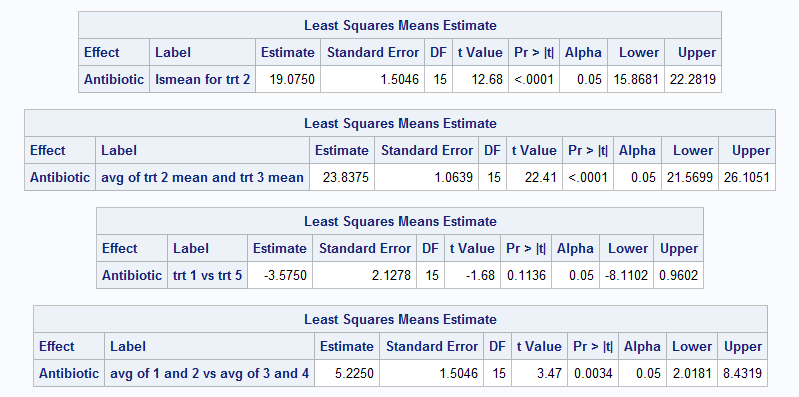
\includegraphics[scale=0.8]{BindFracMixedEstimate}\\
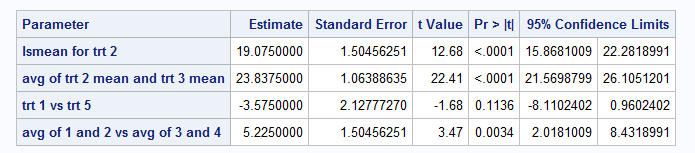
\includegraphics[scale=0.8]{BindFracGLMEstimate}
\end{center}

\newpage

\textbf{Multiple Comparisons Corrections}\\~\\
It is not safe to go carrying out many many significance tests suggested by the data all willy-nilly.  If we do, our \textit{experiment-wise} type I error rate will not be controlled.\\~\\

For instance, we only look at all pairwise comparisons of treatment means if the global p-value is significant.  Thus, these are data driven hypotheses we are testing.  \\~\\

Recall: $\alpha=P(\mbox{Type I Error})$\\
\begin{center}
\begin{tabular}{c|cc}
Decision & $H_0$ true & $H_0$ false\\\hline
Reject $H_0$ & Type I Error & Correct! \\
Fail to Reject $H_0$ & Correct! & Type II Error
\end{tabular}
\end{center}

For a given test, we fix the probability of a type I error to be small (often 0.05) as it is usually considered worse than a type II error.\\~\\
%\color{red}{This is similar to the US justice system where we assume innocence until proven guilty.  For most crimes it is much worse to send an innocent person to jail than to let a guilty person go free}\\~\\
Consider the case with $t=5$ (antibiotic treatments): 
\begin{itemize}
\item the number of pairwise contrasts of the form $\theta=\mu_i-\mu_j$ is $\choose{5}{2}=10$
\item each test has type I error $\alpha=0.05$, but overall what is our experiment-wise type I error rate?
$$\mbox{i.e. P(rejecting at least one null hypothesis that is true)}$$
\item This is called the \textit{experiment-wise} or \textit{family-wise} (fwe) type I error rate.  We should really control this in addition to the type I error for each test!
\end{itemize}

Example:  Is a certain type of coin fair (equal probability of flipping a head and a tail)?
$$H_0: \mbox{Coin fair}, p=0.5~~~~~~~~~~H_A:\mbox{Coin biased}, p\neq 0.5$$
Experiment - flip one of these coins 10 times, if 9 or 10  heads appear or if 9 or 10 tails appear then declare coin biased.\\~\\
Assuming the coin is fair, what is the significance level of this test?

\newpage
 
%\begin{eqnarray*}
%\alpha & = & P(\mbox{Concluding coin is biased})\\
% & = & P(9~heads)+P(9~tails)+P(10~heads)+P(10~tails)\\
%& = & 2*10(1/2)^{10}+2*(1/2)^{10}=0.021
%\end{eqnarray*}
%This is our type I error rate for testing this particular coin (a little smaller than the usual 0.05).\\~\\

Now suppose we have 100 coins of this type and we test each in the same manner.  If the coins were truly fair, how many of the experiments would we expect to conclude we have a biased coin?\\~\\
For a particular coin to come up heads or tails 9-10 times is very unlikely, but seeing any 1 coin of the 100 behave this way would be more likely than not.\\
In fact, \\~\\~\\~\\~\\~\\~\\~\\~\\~\\~\\~\\
%$$P(\mbox{All 100 coins identified as fair})=0.12$$
%$$P(\mbox{At least 1 coin of the 100 is classsified as biased})=0.88$$
%This is why we need to control the fwe rate when we do many data-driven comparisons!\\~\\
\color{blue}{Under the assumption of independence of all tests,
$$\mbox{fwe rate}=P(\mbox{At least 1 type I error})=\alpha^{*}=1-(1-\alpha)^{k}$$
where $k$ is the number of tests being done and $\alpha$ is the significance level used for each test.}\\~\\~\\
\color{black}
Comparisons can be categorized as {\em a priori} or {\em post-hoc}:
\begin{itemize}
\item {\em A priori}: Significance tests which will be carried out without regard to the observed outcome of the experiment.
\item {\em Post-hoc} or data-driven: Significance tests which are suggested by the observed outcome of the experiment.
\end{itemize}

Methods for simultaneous inference for multiple comparisons include (but there are many many of these)
\begin{itemize}
\item Bonferroni (section 9.3)
\item Tukey (section 9.5)
\item Fisher's LSD (don't use this, section 9.4, you should still read this section)
\item Duncan (Not required, used when there is a control treatment, section 9.7)
\item \chef (Not required, section 9.8)
\end{itemize}

\newpage

\textbf{Bonferroni Correction}\\~\\
Suppose interest lies in exactly $k$ linear combinations of means.  \textbf{Bonferroni correction} is to replace the usual $\alpha$ with
$$ \alpha'=\frac{\alpha}{k}$$
By doing so our fwe rate will be less than $\alpha$.\\~\\
We can now create \textbf{simultaneous} CIs.  These are a group of CIs we are $(1-\alpha)$\% confident will \underbar{all} contain their true values.\\~\\
Simultaneous $95\%$ confidence intervals for the $k$ linear combinations of means is given by
$$ a_1 \bar{y}_{1\bullet} + a_2 \bar{y}_{2\bullet} + \cdots + a_t \bar{y}_{t\bullet} \pm t_{\alpha'/2,t(n-1)}\sqrt{MS(E) \sum_{i=1}^{t} \frac{a_i^2}{n_i}} $$
$$\vdots$$ 
$$ k_1 \bar{y}_{1\bullet} + k_2 \bar{y}_{2\bullet} + \cdots + k_t \bar{y}_{t\bullet} \pm t_{\alpha'/2,t(n-1)}\sqrt{MS(E) \sum_{i=1}^{t} \frac{k_i^2}{n_i}} $$
Note: $t_{\alpha'/2,t(n-1)}$ might have to be obtained using software.\\~\\
For the binding fraction example, consider only pairwise comparisons of Chloramphenicol ($\mu_1$):
$$\theta_1 = \mu_1-\mu_2, ~~~~\theta_2 = \mu_1-\mu_3, ~~~~\theta_3 = \mu_1-\mu_4, ~~~~\theta_4 = \mu_1-\mu_5$$
We have $k=4$, $ \alpha'=0.05/k=0.0125,$ and $t_{\alpha'/2,15} = 2.84$.\\~\\
What is the Margin of Error for one of these contrasts?  Find the simultaneous 95\% intervals for the four contrasts.  Which of these antibiotic means differ significantly from the chloramphenicol mean?\\
%\color{red}{The Margin of Errors for the CIs are all the same and are, for example,  
%$$t_{(\alpha'/2,15)}\sqrt{MS(E) \left(\frac{(1)^2}{4} + \frac{(-1)^2}{4}+\frac{0^2}{4} + \frac{0^2}{4} +\frac{0^2}{4}\right)} = 2.84\sqrt{(9.05)\frac{2}{4}} = 6.043 $$
%so that \textit{simultaneous} $95\%$ confidence intervals for $\theta_1,\theta_2,\theta_3,\theta_4$ are
%$$\mbox{for }\theta_1:~~~\bar{y}_{1\bullet}-\bar{y}_{2\bullet} \pm 6.043 = 27.800-19.075 \pm 6.043 = (2.682, 14.768)$$
%$$\mbox{for }\theta_2:~~~\bar{y}_{1\bullet}-\bar{y}_{3\bullet} \pm 6.043 = 27.800-28.600 \pm 6.043 = (-6.836, 5.236)$$
%$$\mbox{for }\theta_3:~~~\bar{y}_{1\bullet}-\bar{y}_{4\bullet} \pm 6.043 = 27.800-~7.825 \pm 6.043 = (13.939, 26.011)$$
%$$\mbox{for }\theta_4:~~~\bar{y}_{1\bullet}-\bar{y}_{5\bullet} \pm 6.043 = 27.800-31.375 \pm 6.043 = (-9.611, 2.461)$$
%}

\newpage

\textbf{Tukey-Kramer Correction (or just Tukey)}\\~\\
Tukey's correction is the best (most powerful) method when making inference on \textbf{all pairwise} contrasts in balanced designs. That is, for simple contrasts of the form
$$ \theta=\mu_j-\mu_k$$
it will tend to have a lower type II error rate in these cases than other multiple comparison corrections.  (It has a greater chance of detecting differences i.e. is more powerful.)
\begin{itemize}
\item Uses multipliers from a distribution called the `studentized range distribution'
\item Denoted $q(\alpha,t,t(n-1))$
\end{itemize}
For a balanced design, {\bf simultaneous} $95\%$ confidence intervals for $\theta=\mu_j-\mu_k$ are given by
\begin{eqnarray*}
\hat{\theta}&\pm& \frac{q(\alpha,t,t(n-1))}{\sqrt{2}} \hat{SE}(\hat{\theta})\\
\bar{y}_{j+}-\bar{y}_{k+}&\pm& \frac{q(\alpha,t,t(n-1))}{\sqrt{2}}\sqrt{MS(E)\left(\frac{1}{n}+\frac{1}{n}\right)}\\
\bar{y}_{j+}-\bar{y}_{k+}&\pm& q(\alpha,t,t(n-1))\sqrt{\frac{MS(E)}{n}}
\end{eqnarray*}

\textbf{How to do these multiple comparison corrections in SAS?}
\begin{itemize}
\item Bonferonni can be done by manually changing the $\alpha$ level SAS uses.  For the example above, $\alpha'=0.05/4=0.0125$:
\begin{small}
\begin{verbatim}
proc glm data=binding;  class antibiotic;
model bindfrac=antibiotic/clparm alpha=0.0125;  *Can drop intercept since it has 0 coefficient;
estimate 'theta 1' antibiotic 1 -1;             *Note these are different thetas than previous;
estimate 'theta 2' antibiotic 1 0 -1;
estimate 'theta 3' antibiotic 1 0 0 -1 0;
estimate 'theta 4' antibiotic 1 0 0 0 -1;   run;

proc mixed data=binding; class antibiotic;
model bindfrac=antibiotic; 
lsmestimate antibiotic 'theta 1' [1,1] [-1,2],
                       'theta 2' [1,1] [-1,3],
                       'theta 3' [1,1] [-1,4],
                       'theta 4' [1,1] [-1,5]/cl adjust=bon;  run;
\end{verbatim}
\end{small}

\item Tukey correction is an option you ask for:
\begin{small}
\begin{verbatim}
proc glm data=binding; class antibiotic;
model bindfrac=antibiotic;
lsmeans antibiotic/pdiff adjust=tukey cl;  run;

proc mixed data=binding; class antibiotic;
model bindfrac=antibiotic;
lsmeans antibiotic/pdiff adjust=tukey cl;  run;
\end{verbatim}
\end{small}
\end{itemize}

\newpage

Bonferroni GLM output:
\begin{center}
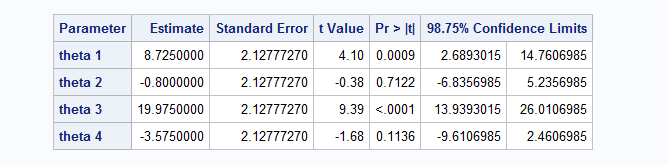
\includegraphics[scale=0.8]{BindFracBon}
\end{center}
Bonferroni Mixed output:
\begin{center}
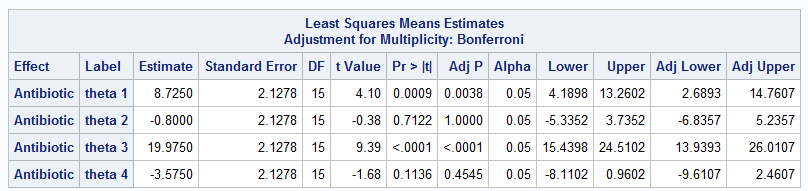
\includegraphics[scale=0.8]{BindFracBonMixed}
\end{center}

Tukey Mixed output:
\begin{center}
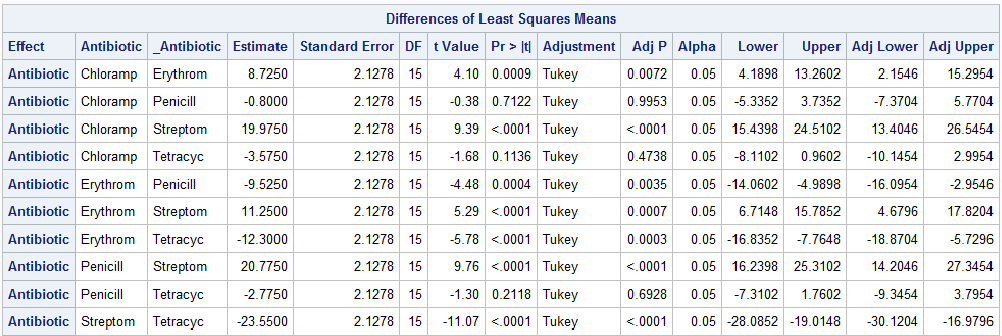
\includegraphics[scale=0.65]{BindFracTukeyMixed}
\end{center}

\newpage

Tukey GLM output:
\begin{flushleft}
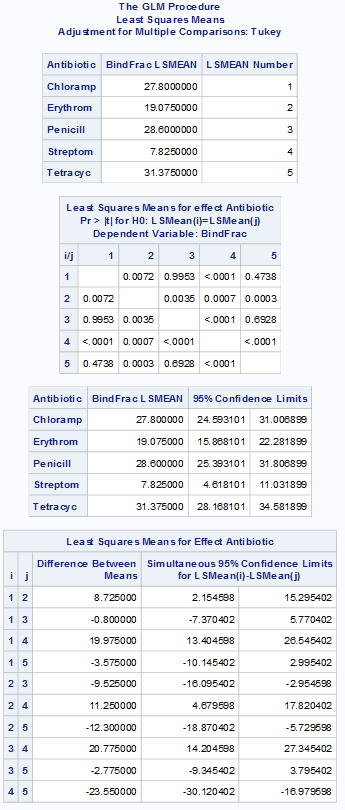
\includegraphics[scale=0.8]{BindFracTukey}
\end{flushleft}

\newpage

\Large\textbf{Independent Contrasts}\large\\

So, what else can we do with contrasts?\\~\\

Consider a contrast $\theta$, then
$$\theta=c_{1}\mu_{1}+c_{2}\mu_{2}+...+c_{t}\mu_{t}$$
where $\sum_{i=1}^{t}c_i=0$.  The point estimate of a contrast is
$$\hat{\theta}=c_{1}\bar{y}_{1+}+c_{2}\bar{y}_{2+}+...+c_{t}\bar{y}_{t+}$$
and the estimated variance is given by
$$\hat{Var}(\hat{\theta})=MS(E)\sum_{i=1}^{t}\frac{c_i^2}{n_i}$$
Recall: The idea behind ANOVA is that we partition $SS(Tot)$ (with df=N-1) into independent components $SS(Trt)$ and $SS(E)$ (whose df add up to N-1).\\~\\
Similarly, we can take $SS(Trt)$ and partition it into $t-1$ independent contrasts each with 1 df.  How you ask??\\~\\

\textbf{Orthogonal contrasts}:\\
Let 
$$\theta_1=\sum_{i=1}^{t}c_i\mu_i \mbox{    and    }\theta_2=\sum_{i=1}^{t}d_i\mu_i$$
be two contrasts.  $\theta_1$ and $\theta_2$ are \textbf{orthogonal} if 
$$c_1d_1+c_2d_2+...+c_td_t=\sum_{i=1}^{t}c_id_i=0$$
(for balanced designs).\\~\\
If two contrasts are orthogonal, then one contrast conveys no information about the other contrast.  Hence we can break up $SS(Trt)$ into completely separate sources.\\~\\
A set of $k$ contrasts is mutually orthogonal if all pairs are orthogonal. As we have $t-1$ df, we can break $SS(Trt)$ into at most $t-1$ orthogonal contrasts.\\~\\
This will allow us to attribute a certain amount of variation to given contrasts, which in turn will represent something of interest to you the researcher.

\newpage

Examples:\\
$ (-1,1,0,0,0) \mbox{ and } (0,0,-1,1,0) \mbox{ orthogonal ?}$\\~\\~\\
$ (1,-1/2,-1/2,0,0) \mbox{ and } (0,0,0,-1,1) \mbox{ orthogonal ?}$\\~\\~\\
$ (-1,1,0,0,0) \mbox{ and } (0,-1,1,0,0) \mbox{ orthogonal ?}$\\~\\~\\
Due to the joint normality of our data, \textbf{orthogonality implies independence}!  \\~\\

\textbf{Sums of squares for contrasts}\\
Recall we are going to partition $SS(Trt)$ into $t-1$ independent contrasts, each will have its own sum of squares.  The sums of squares for a contrast are defined as
$$ SS(\hat\theta)=\frac{\hat\theta^2}{\left(\frac{c_1^2}{n_1}+\cdots+\frac{c_t^2}{n_t}\right)}=\frac{\hat\theta^2}{\left(\sum_{i=1}^{t}\frac{c_i^2}{n_i}\right)}$$
This contrast has 1 df associated with it.\\~\\

\textbf{Alternative (but equivalent) test for a contrast}\\
Previously, we saw that we could test a linear combination (and hence a contrast) via a t-test.  Now, we can define 
$$MS(\hat{\theta})=SS(\hat{\theta})/1=SS(\hat{\theta})$$
and can then test
$$H_0:\theta=0~~~~vs~~~~H_A:\theta\neq 0$$
using the F-statistic
$$F=\frac{MS(\hat{\theta})}{MS(E)}\sim F_{1,t(n-1)}$$
Compare this to the $t$-test done earlier for testing a contrast equal to 0
$$t=\frac{\hat{\theta}-0}{\hat{SE}(\hat{\theta})}\sim t_{t(n-1)}$$
If we square a $t$ stat we get an $F$ stat!
%$$t^2=\left(\frac{\hat{\theta}}{\hat{SE}(\hat{\theta})}\right)^2=\frac{\left(\hat{\theta}\right)^2}{\hat{Var}(\hat{\theta})}=\frac{\left(\hat{\theta}\right)^2}{MS(E)\sum_{i=1}^{t}\frac{c_i^2}{n}}=\frac{MS(\hat{\theta})}{MS(E)}$$~\\

\newpage

\textbf{Simultaneous test for contrasts}\\
We can also test multiple orthogonal contrasts all equal to 0 at once
$$H_0:\theta_1=\theta_2=...=\theta_k=0~~~~vs~~~~H_A:\mbox{At least 1 }\theta\neq 0$$
using the F-statistic
$$F=\frac{\frac{SS(\hat{\theta_1})+SS(\hat{\theta_2})+...+SS(\hat{\theta_k})}{k}}{MS(E)}\sim F_{k,t(n-1)}$$
~\\~\\
How to relate this to $SS(Trt)$? \\
Generally, if $\theta_1,\theta_2,...,\theta_{t-1}$ are $t-1$ mutually orthogonal contrasts then
$$ SS(Trt)=SS(\hat\theta_1)+SS(\hat\theta_2)+\cdots+SS(\hat\theta_{t-1})$$
and $df_{Trt}=df_{\hat\theta_1}+...+df_{\hat\theta_{t-1}}=1+...+1=t-1$\\~\\
Notice, testing all $t-1$ contrasts equal to 0 is equivalent to testing our global $F$-test!\\~\\~\\~\\

Again consider the Binding Fraction data.  In this case we have $5-1=4$ df for treatment.  Consider the following set of 4 mutually orthogonal contrasts:
\begin{eqnarray*}
\theta_1&=&(-2~~-1~~~~0~~~~~1~~~~2)\\
\theta_2&=&(2~~~~-1~-2~~-1~~~~2)\\
\theta_3&=&(-1~~~~~2~~~~0~~-2~~~~1)\\
\theta_4&=&(1~~~~-4~~~~6~~-4~~~~1)
\end{eqnarray*}
Since these are mutually orthogonal, they are all independent.\\

\newpage

Let's use SAS to get estimates.  Test for $\theta_4=0$ using both the $t$ and $F$ tests.  Then show that $SS(Trt)=SS(\theta_1)+SS(\theta_2)+SS(\theta_3)+SS(\theta_4)$ and conduct the global $F$ test.\\
\begin{small}
\begin{verbatim}
proc glm data=binding; class antibiotic; model bindfrac=antibiotic;
contrast 'theta 1' antibiotic -2 -1 0 1 2;
contrast 'theta 2' antibiotic 2 -1 -2 -1 2;
contrast 'theta 3' antibiotic -1 2 0 -2 1;
contrast 'theta 4' antibiotic 1 -4 6 -4 1; run;



proc mixed data=binding; class antibiotic; model bindfrac=antibiotic;
lsmestimate antibiotic 'theta 1' [-2,1] [-1,2] [0,3] [1,4] [2,5],
'theta 2' [2,1] [-1,2] [-2,3] [-1,4] [2,5], 
'theta 3' [-1,1] [2,2] [0,3] [-2,4] [1,5], 
'theta 4' [1,1] [-4,2] [6,3] [-4,4] [1,5]; run;

*I've done the estimate statements in proc mixed, but you could do them in glm instead;
*Also, we may want to do a multiple comparison correction depending on 
\end{verbatim}
\end{small}
Note the equivalence of the p-value for a contrast and for an estimate statement.
\begin{flushleft}
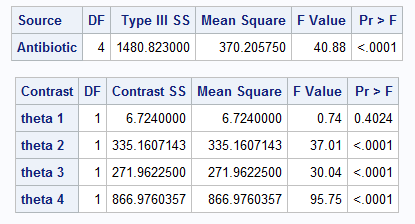
\includegraphics[scale=0.75]{BindFracContrastSS}\\
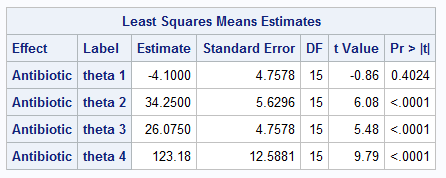
\includegraphics[scale=0.7]{BindFracContrastMixed}
\end{flushleft}

\newpage

\textbf{Another example}\\
Data consists of the number of contaminants in IV fluids made by $t=3$ pharmaceutical companies
\begin{center}
\begin{tabular}{c|ccc|} \hline
&Cutter & Abbott & McGaw \\ \hline
$y_{i1}$&255 & 105 & 577 \\
$y_{i2}$&264 & 288 & 515 \\
$y_{i3}$&342 & 98 & 214 \\
$y_{i4}$&331 & 275 & 413 \\
$y_{i5}$&234 & 221 & 401 \\
$y_{i6}$&217 & 240 & 260 \\ \hline
$\bar{y}_{i\bullet}$ &273.8 & 204.5 & 396.7 \\ \hline
\end{tabular}
\end{center}
\begin{center}
\begin{tabular}{|c|c|c|c|c|}  \hline
& & Sum of & Mean & \\
Source & d.f. & squares & Square & F \\ \hline
Treatments (pharmacy) & $2$ & 113646 & 56823 & 5.81\\
Error & $15$ & 146753 & 9784 & \\
Total & 17 & 260400 & & \\ \hline
\end{tabular}
\end{center}
Consider the following 2 contrasts:
$$ \theta_1 = \mu_M-\mu_A \ \ \ \mbox{ and }\ \ \ \theta_2=\mu_C-\frac{\mu_M+\mu_A}{2}$$
Which levels of the factor will each of these be in SAS? \\~\\~\\~\\
Rewrite these contrasts in terms of $\mu_1$, $\mu_2$, and $\mu_3$.\\~\\~\\~\\~\\~\\
Are these contrasts orthogonal (and thus independent)?\\~\\~\\~\\~\\
Use the output to compute $SS(\hat\theta_1)$ and $SS(\hat\theta_2)$.  What should these add up to and why?

\newpage

\begin{small}
\begin{verbatim}
proc glm data=pharm; class company; model contam=company;
contrast 'McGaw vs Abbot' company -1 0 1;
estimate 'McGaw vs Abbot'  company -1 0 1;
contrast 'Cutter vs avg of McGaw and Abbot' company -1 2 -1;
estimate 'Cutter vs avg of McGaw and Abbot' company -1 2 -1/divisor=2; run;
\end{verbatim}
\end{small}
 Note: We should really do a multiple comparison correction for our two contrasts.  Bonferonni is easiest, compare our p-values to $0.05/2=0.025$.
\begin{flushleft}
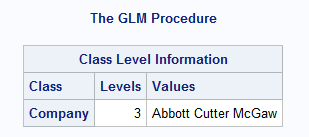
\includegraphics[scale=0.7]{PharmGLM1}\\
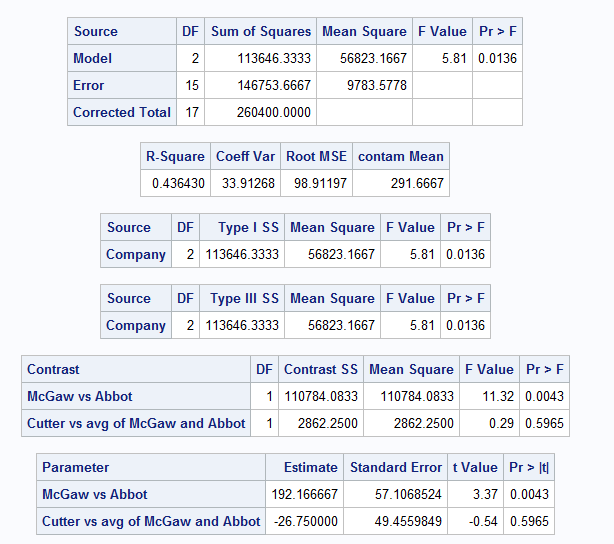
\includegraphics[scale=0.7]{PharmGLM2}\\

\includegraphics[scale=0.7]{PharmGLM3}
\end{flushleft}

For another good example, see page 457, example 9.3.



